\chapter{Lý Thuyết}
\label{chap:background}
\graphicspath{{Chapter3/Figs/}}

\begin{chapabstract}
Đầu tiên, chương \ref{chap:background} trình bày các nền tảng lý thuyết được sử dụng trong đề tài, bao gồm các loại malware, PE file format và các kiến thức lý thuyết khác về học máy. Sau đó, các thước đo đánh giá và framework sử dụng cho thuật toán học máy đã được sử dụng trong việc implement thuật toán sẽ được giới thiệu.
\end{chapabstract}

\section{Malware Types}
\label{sec:malware}

Phân loại là cách tuyệt vời để hiểu rõ hơn về phần mềm độc hại. Một số loại phổ biến nhất bao gồm: adware, bots, rootkits, spyware, Trojan horses, viruses, and worms \cite{neil2012common}.

\subsection{Virus}

Virus là một dạng phần mềm độc hại có khả năng sao chép chính nó và lây lan sang các máy tính khác bằng cách đính kèm vào các ứng dụng khác nhau và thực thi khi người dùng khởi chạy một trong số đó. Virus cũng có thể lây lan qua các tài liệu, tệp kịch bản và lỗ hổng tập lệnh script (cross-site scripting vulnerabilities) trong các ứng dụng web. Một số ví dụ nổi tiếng của virus trong những năm qua là virus Concept, virus Chernobyl (còn được gọi là CIH), virus Anna Kournikova, Brain và RavMonE.exe.

\subsection{Worm}

Worm là một phần mềm độc lập sao chép mà không cần nhắm mục tiêu và lây nhiễm các tệp cụ thể. Hãy nghĩ về worm như các chương trình nhỏ tự sao chép bản thân và phá hủy dữ liệu. Nó thường nhắm vào các tập tin hệ điều hành và làm việc cho đến khi ổ đĩa trở nên trống rỗng. Một số ví dụ bao gồm Melissa, Morris, Mydoom, Sasser và Blaster.

\subsection{Trojan}

Trojan là một ứng dụng độc hại giả dạng bản thân để trông hữu ích và đánh lừa người dùng tải xuống và cài đặt. Trojan có thể cung cấp quyền truy cập từ xa vào một máy tính bị nhiễm để kẻ tấn công có thể lấy cắp dữ liệu, cài đặt thêm phần mềm độc hại, theo dõi hoạt động của người dùng, v.v. Các ví dụ đáng chú ý cũng bao gồm những con Trojan được phát triển bởi các cơ quan chính phủ Hoa Kỳ như FBI và NSA. Những cái tên như Magic Lantern, FinFisher, Netbus, Beast, Gh0st RAT, Clickbot.A, và Zeus đã trở thành lý do của kinh sự kinh hoàng. Tương tự  một trojan trên Android được phát hiện vào năm 2015, tên là Shedun, là một trong nhiều malware nhắm đến mục tiêu là thiết bị di động.

\subsection{Ransomware}

Ransomware, một trong những phần mềm độc hại nhất và liên tục xuất hiện, là một loại phần mềm độc hại thường giam giữ một hệ thống máy tính và yêu cầu một khoản tiền chuộc, ví dụ như chặn truy cập vào dữ liệu của nạn nhân hoặc đe dọa công khai nội dung của nó. Tệ hơn nữa, không có gì đảm bảo rằng việc thanh toán sẽ nhận được quyền truy cập vào dữ liệu hoặc ngăn không cho công khai dữ liệu nhạy cảm. Các ransomware nổi tiếng như Reveton, CryptoLocker, CryptoWall, và gần đây hơn, cuộc tấn công WannaCry năm 2017, đã gây ra không một lượng không nhỏ tổn hại \cite{chen2017automated}.

\subsection{Rootkit}

Rootkit là một tập hợp các phần mềm được thiết kế đặc biệt để cho phép phần mềm độc hại xâm nhập hệ thống của bạn và thu thập thông tin. Những công việc này ở chế độ nền để người dùng có thể không nhận thấy bất kỳ điều gì khác biệt. Nhưng bên trong môi trường, một rootkit sẽ cho phép một số loại phần mềm độc hại xâm nhập vào hệ thống. Rootkit đầu tiên có được danh tiếng trên Windows là NTRootkit vào năm 1999, nhưng phổ biến nhất là vụ bê bối Sony BMG copy protection rootkit scandal đã làm rung chuyển công ty trong năm 2005 \cite{bruce2005sony}.

\subsection{Adware}

Mặc dù phần mềm hỗ trợ quảng cáo (adware) hiện phổ biến hơn nhiều, adware đã được liên kết với phần mềm độc hại trong một thời gian dài. Trong khi phần mềm quảng cáo có thể tham chiếu đến bất kỳ ứng dụng nào được quảng cáo hỗ trợ, phần mềm quảng cáo độc hại thường hiển thị quảng cáo dưới dạng cửa sổ bật lên và ngăn cửa sổ không thể đóng. Đó có lẽ là phần mềm độc hại hiệu quả nhất và ít nguy hiểm nhất, được thiết kế với mục đích cụ thể là quảng bá quảng cáo trên máy tính của bạn.

\subsection{Bot}

Bots là các chương trình phần mềm được tạo ra để thực hiện các hoạt động cụ thể một cách tự động. Trong khi một số bot được tạo ra cho mục đích vô hại, nó ngày càng trở nên phổ biến để xem bot đang được sử dụng độc hại. Bots có thể được sử dụng trong botnet (tập hợp các máy được kiểm soát bởi các bên thứ ba) để thực hiện các tấn công từ chối dịch vụ phân tán, gửi spam và ăn cắp dữ liệu.

\section{PE File Format}
\label{sec:pe-file}

Định dạng tệp Portable Executable (PE) mô tả định dạng thực thi chiếm ưu thế cho hệ điều hành Microsoft Windows và bao gồm tệp thực thi, thư viện liên kết động (DLL) và tệp phông chữ FON. Định dạng này hiện được hỗ trợ trên Intel, AMD và các biến thể của kiến trúc bộ lệnh ARM.

Tệp PE bao gồm một số header và section mô tả dynamic linker biết cách ánh xạ tệp vào bộ nhớ. Một tệp thực thi bao gồm một số vùng khác nhau, mỗi vùng đòi hỏi sự bảo vệ bộ nhớ khác nhau; do đó, bắt đầu của mỗi phần phải được căn chỉnh với một khung trang. Thông thường, các header bao gồm Common Object File Format (COFF) file header chứa các thông tin cần thiết như machine type, file type (DLL, EXE, OBJ), số lượng sections, số lượng symbols, v.v. Optional header xác định linker version, kích thước của code, kích thước của initialized data và uninitialized data, entry point address, v.v. Các data directory nằm optional header cung cấp con trỏ đến section chứa nó. Những section này bao gồm tables for exports, imports, resources, exceptions, debug information, certificate information, và relocation tables. Do đó, định dạng PE cung cấp một bản tổng hợp các thông tin hữu ích của một tệp thực thi \cite{shafiq2009pe}. 

\begin{figure}[H] 
\centering    
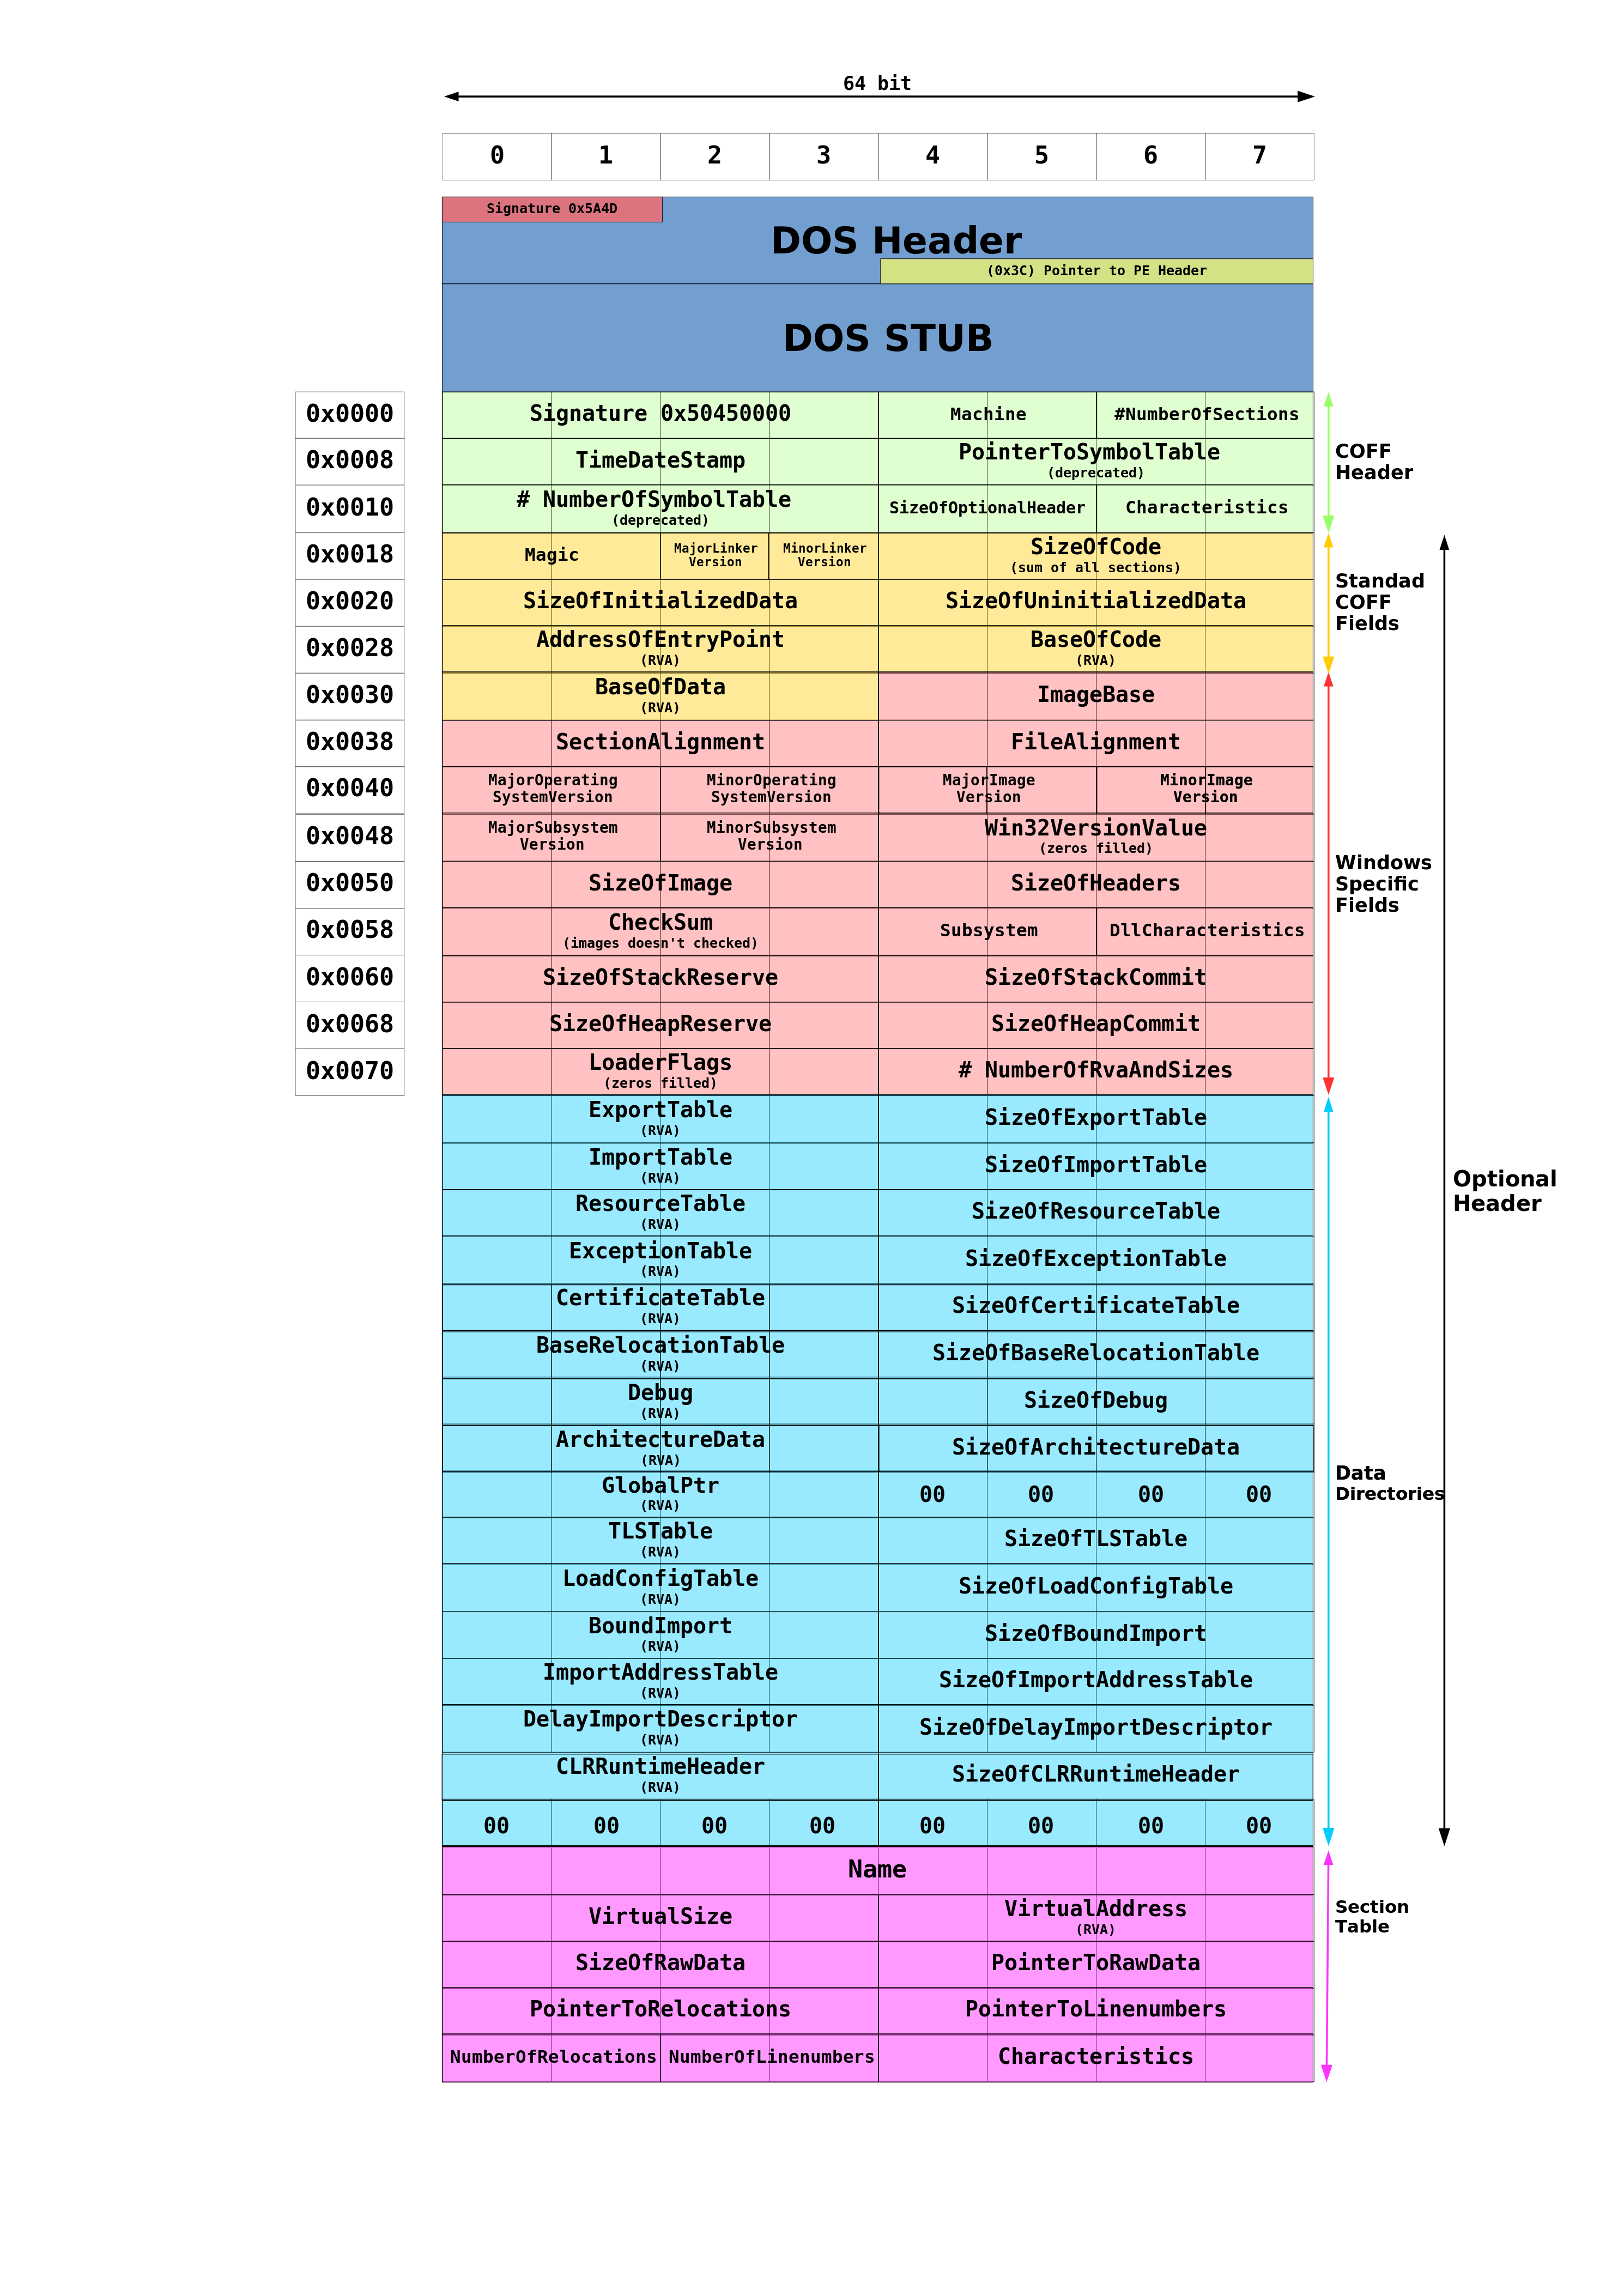
\includegraphics[width=1.0\textwidth]{Portable_Executable_32_bit.png}
\caption{Kết cấu của tệp Portable Executable 32-bit \cite{wikipefile}}
\label{fig:pe32bit}
\end{figure}

Các section của PE chứa code và initialized data mà Windows loader sẽ ánh xạ vào vùng thực thi hoặc vùng bộ nhớ đọc/viết, cũng như là imports, exports, và resources được định nghĩa trong tệp. Mỗi section chưa một header sẽ chỉ định kích cỡ và địa chỉ. Import address table chỉ thị loader function nào sẽ được import tĩnh.Resources section có thể chứa các resource cần thiết cho người dùng như là: cursors, fonts, bitmaps, icons, menus, v.v. Một tập PE cơ bản thường sẽ có \verb|.text| code section và một hoặc nhiều data section (\verb|.data|, \verb|.rdata| hoặc \verb|.bss|). Relocation tables thường được chứa trong \verb|.reloc| section, và được sử dụng bởi Windows loader để reassign base address từ the executable’s preferred base. Section \verb|.tls| thường chứa special thread local storage (TLS) structure cho việc luuaw trữ các biến riêng cho thread. Các section name được gọi ngẫu nhiên từ phía Windows loader, nhưng các tên cụ thể đã được chấp nhận bởi tiền lệ và phổ biến rộng rãi.

\section{Machine Learning}

\subsection{Tổng quan}
\label{ssec:machine-learning-intro}

Trong những năm gần đây, hầu hết các nghiên cứu và tiến bộ sản xuất đều xuất phát từ tiểu ngành cuar Trí tuệ nhân tạo mang tên Machine Learning. Nguyên tắc Machine Learning rất đơn giản; Machine Learning là một phương pháp mà máy tính tìm thấy các pattern từ dữ liệu và đưa các pattern đó vào các ứng dụng. Sau đó, ứng dụng có thể có được thông tin chi tiết về dữ liệu mới dựa trên sự giống nhau với các pattern được xác định \cite{martin2016machine}.

\begin{figure}[htbp!] 
\centering    
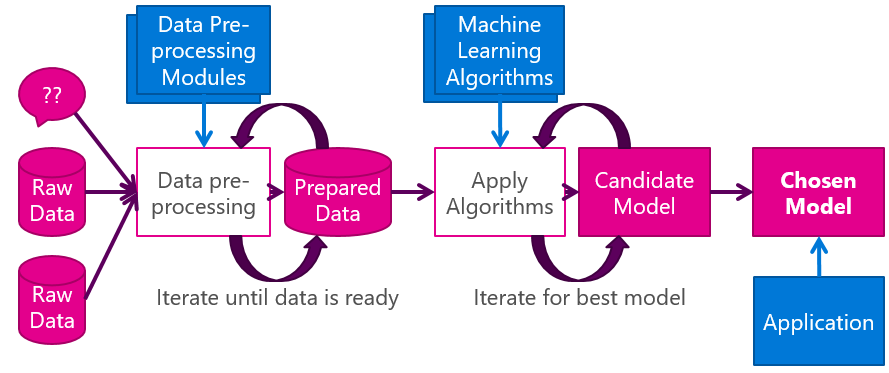
\includegraphics[width=1.0\textwidth]{MLProcess.png}
\caption{Quy trình học máy \cite{martin2016machine}}
\label{fig:ml-process}
\end{figure}

Hãy xem xet các công việc chung (Hình \ref{fig:ml-process}) của một quy trình học máy:

\begin{itemize}
\item Mục tiêu chính của quá trình này là xác định một mô hình. 
Mô hình là điều chính mà ứng dụng có thể gửi yêu cầu để có được thông tin chi tiết về dữ liệu mới.
\item Trước khi đi vào thử nghiệm Machine Learning, chúng ta phải xác định mục đích và cách đánh giá kết quả.
\item Quá trình bắt đầu với việc chuẩn bị dữ liệu. 
Dữ liệu được chuẩn bị là một hoặc nhiều tập dữ liệu đã được xử lý trước (định dạng, làm sạch và lấy mẫu) để sẵn sàng áp dụng thuật toán Machine Learning. 
Chuẩn bị dữ liệu có nghĩa là làm cho dữ liệu có hình dạng tốt nhất để rút ra kết luận khoa học.
\item Bước tiếp theo là áp dụng một hoặc nhiều thuật toán Máy học tạo ra một Mô hình, đó là một quá trình lặp lại và chúng ta có thể lặp lại việc kiểm tra các thuật toán khác nhau cho đến khi chúng ta đạt được một mô hình đủ để đạt được mục đích.
\end{itemize}

Không phải tất cả các vấn đề đều là có thể áp dụng giải pháp học máy. 
Vấn đề này phải là một vấn đề có thể được giải quyết bằng dữ liệu, và có đủ số lượng dữ liệu có liên quan để được sử dụng. 
Như chúng ta sẽ thấy, nhiều vấn đề bảo mật phù hợp với yêu cầu này cực kỳ tốt.

\subsection{Supervised Learning}
\label{ssec:supervised-learning}

Các thuật toán học được giám sát (supervised learning) đưa ra dự đoán dựa trên một tập hợp mẫu, ví dụ: giá cổ phiếu trong lịch sử có thể được sử dụng để đoán giá tương lai.
Thuật toán học được giám sát tìm kiếm các pattern trong dữ liệu được gắn nhãn.
Nó có thể sử dụng bất kỳ thông tin nào có thể có liên quan và mỗi thuật toán sẽ tìm các loại pattern khác nhau.
Sau khi thuật toán đã phát hiện pattern tốt nhất có thể, nó sử dụng pattern đó để đưa ra các dự đoán cho dữ liệu không được dán nhãn.

Khi dữ liệu đang được sử dụng để dự đoán danh mục, học tập được giám sát được gọi là phân loại, ví dụ: chỉ định hình ảnh làm hình ảnh của chú mèo hoặc chó. Khi chỉ có hai lựa chọn, nó được gọi là phân loại hai lớp, nhị thức hoặc nhị phân. Khi có nhiều danh mục hơn, vấn đề này được gọi là phân loại nhiều lớp.

\subsection{Feature Extraction}

Như đã đề cập trong phần \ref{ssec:machine-learning-intro},chúng ta nên trích xuất các thuộc tính từ dữ liệu đầu vào để chúng ta có thể đưa nó vào thuật toán. Ví dụ, trong các trường hợp hình ảnh, dữ liệu có thể được biểu diễn dưới dạng giá trị RGB của mỗi pixel.

Các thuộc tính như vậy được gọi là \textbf{các đặc trưng}, và ma trận được gọi là vector đặc trưng. Quá trình trích xuất đặc trưng từ các tệp gọi là feature extraction. Mục đích của việc feature extraction là để có được một tập hợp dữ liệu nhiều thông tin và không dư thừa.

Các đặc trưng phải thể hiện thông tin cần thiết và có liên quan về tập dữ liệu của chúng ta vì chúng ta không thể đưa ra dự đoán chính xác mà không có nó.
Đó là lí do tại sao feature extraction thường là một nhiệm vụ không rõ ràng và phụ thuộc vào lĩnh vực cụ thể, đòi hỏi nhiều thử nghiệm và nghiên cứu.

Một yêu cầu quan trọng khác đối với một bộ đặc trưng phù hợp là không dư thừa.
Việc xuất hiện các đặc trưng dư thừa, cụ thể là các yếu tố nằm ngoài vùng thông tin hoặc các yếu tố không liên quan, có thể làm cho thuật toán thiên vị, theo đó là việc cung cấp kết quả không chính xác.

\subsection{Classification, Regression và Thresholding}

\textbf{Classification} là công việc xấp xỉ hàm ánh xạ ($f$) từ các biến đầu vào ($X$) để đưa ra biến đầu ra rời rạc ($y$). 
Các biến đầu ra thường được gọi là nhãn hoặc danh mục. 
Hàm ánh xạ dự đoán lớp hoặc nhóm cho một quan sát đã cho.
Ví dụ: một email có thể được phân loại là thuộc một trong hai loại: "spam" và "không phải spam".

\textbf{Regression} là công việc xấp xỉ hàm ánh xạ ($f$) từ các biến đầu vào ($X$) để đưa ra biến đầu ra liên tục ($y$). 
Biến đầu ra là giá trị thực, chẳng hạn như giá trị số nguyên hoặc số thực.
Đây thường là số định lượng, chẳng hạn như số lượng và kích cỡ.
Ví dụ: một căn nhà có thể được dự đoán sẽ bán cho một giá trị đô la cụ thể, có thể trong phạm vi từ 100,000 đô la đến 200.000 đô la.

Các vấn đề classification thường khác các vấn đề regression.
Classification là công việc dự đoán nhãn lớp rời rạc, còn regression là công việc dự đoán số lượng liên tục. 
Tuy nhiên, có một số chồng chéo giữa các thuật toán để phân loại và hồi quy.
Ví dụ, chúng ta có thể sử dụng xác suất, được trả về từ regression, trực tiếp hoặc chuyển nó thành một giá trị nhị phân. 
Để ánh xạ một giá trị logistic regression sang danh mục nhị phân, chúng ta phải định nghĩa một \textbf{classification threshold} (còn gọi là decision threshold).
Có thể giả định rằng classification threshold luôn là 0,5, nhưng threshold phụ thuộc vào các vấn đề cụ thể và do đó đây là giá trị mà chúng ta phải điều chỉnh.

\subsection{Ensemble, Bagging và Boosting}

Khi chúng ta cố gắng dự đoán biến mục tiêu sử dụng bất kỳ phương pháp học máy nào, nguyên nhân hàng đầu của sự khác biệt trong giá trị ban đầu và được dự đoán là noise, variance, và bias. Ensemble giúp giảm hai yếu tố phía sau.

Một ensemble là một tập hợp các mô hình dự đoán để cùng đưa ra dự đoán cuối cùng. Lý do chính là nhiều mô hình dự đoán khác nhau cố gắng dự đoán cùng một biến mục tiêu sẽ thực hiện một công việc tốt hơn so với bất kỳ một đơn lẻ nào. Kỹ thuật ensemble được phân loại thêm vào Bagging và Boosting.

Bagging là một kỹ thuật ensemble đơn giản bằng cách xây dựng nhiều mô hình độc lập và kết hợp chúng bằng những phương pháp lấy trung bình (ví dụ như, lấy trọng số trung bình, đa số phiếu bình chọn hoặc lấy trung bình bình thường). Chúng tôi thường sử dụng tập nhỏ ngẫu nhiên của dữ liệu cho mỗi mô hình, để tất cả các mô hình có chút khác biệt với nhau. Mỗi quan sát có cùng xác suất xuất hiện trong tất cả các mô hình. Bởi vì kỹ thuật này dùng nhiều dự báo không tương quan để tạo ra một mô hình cuối cùng, nó làm giảm lỗi bằng cách giảm variance. Một ví dụ nổi tiếng của kỹ thuật bagging ensemble là Random Forest (được đề cập ở phần \ref{ssec:random-forest}).

Boosting là một kỹ thuật ensemble technique mà các mô hình được xây dựng một cách tuần tự. Kỹ thuật này áp dụng logic trong đó mô hình dự báo phía sa học hỏi từ những sai lầm của những mô hình trước đó. Theo đó, các quan sát có xác suất không đồng đều xuất hiện trong các mô hình tiếp theo. Mô hình dự báo có thể chọn từ nhiều thuật toán như decision trees, regressors, classifiers, v.v. Bởi vì các mô hình phía sau học tập từ những lỗi sai của mô hình phía trước, nó sử dụng ít số iteration để đạt được độ chính xác đã có. Những chúng ta phải chọn điểm dừng phù hợp, hoặc nó có thể dẫn đến việc overfitting trên tập dữ liệu huấn luyện. Gradient Boosting Decision Tree, được đề cập trong phần \ref{ssec:gbdt}, là một ví dụ của kỹ thuật này.

\section{Các phương pháp Machine Learning}

\subsection{Decision Tree}
\label{ssec:decision-tree}

Ngay từ tên của thuật toán, cây quyết định là cấu trúc dữ liệu có cấu trúc của cây. Bộ dữ liệu đào tạo được sử dụng để tạo ra cây, cây này được sử dụng để đưa ra các dự đoán về dữ liệu thử nghiệm. Trong thuật toán này, mục đích là đạt được kết quả chính xác nhất với số lượng ít nhất các quyết định phải được đưa ra. Chúng ta có thể sử dụng cây quyết định có thể cho cả vấn đề phân loại và hồi quy. Bảng \ref{table:decision-tree} đưa ra một ví dụ.

\begin{table}[ht]
\caption{Một ví dụ về Decision Tree}
\centering
\label{table:decision-tree}
\begin{tabular}{c l l c c c c}
\hline
Id & Name                       & Sex    & Age  & SibSp & Survived \\	
\hline
1  & Braund, Mr. Owen Harris    & male   & 22.0	& 1     & 0	\\
2  & Cumings, Mrs. John Bradley & female & 38.0	& 1     & 1	\\
3  & Heikkinen, Miss. Laina	    & female & 26.0	& 0     & 1 \\
...& ...                        & ...    & ...  & ...   & ... \\ 
\hline 
\end{tabular}
\end{table}

\begin{figure}[htbp!] 
\centering    
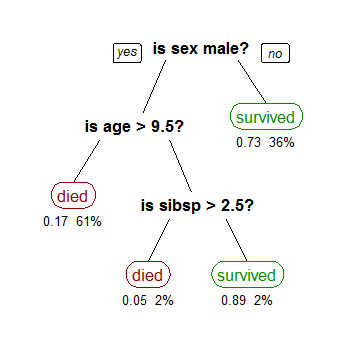
\includegraphics[width=0.5\textwidth]{decesion_tree.png}
\caption{Một ví dụ về Decision Tree \cite{wikidecesiontree}}
\label{fig:decision-tree}
\end{figure}

Trong Hình \ref{fig:decision-tree}, mô hình được đào tạo dựa trên tập dữ liệu và bây giờ có thể phân loại hành khách trong Titanic là sống sót hay không. Cây bao gồm các nút quyết định và các nút lá, và các nút quyết định có thể có nhiều nhánh dẫn đến các nút lá. Nút lá đại diện cho các quyết định hoặc phân loại. Nút đầu tiên đầu tiên được gọi là nút gốc.

Phương pháp cây quyết định đã trở nên phổ biến vì tính đơn giản của nó. Nó có thể xử lý tốt với các bộ dữ liệu lớn và có thể xử lý nhiễu trong bộ dữ liệu rất tốt. Một ưu điểm khác là không giống như các thuật toán khác, chẳng hạn như SVM hoặc KNN, cây quyết định hoạt động trong một hộp màu trắng, có nghĩa là chúng ta có thể thấy kết quả thu được như thế nào và quyết định nào dẫn đến nó.

\subsection{Random Forest}
\label{ssec:random-forest}

Random Forest là một trong những thuật toán học máy phổ biến nhất. Nó hầu như không có đòi hỏi việc chuẩn bị dữ liệu và mô hình hóa nhưng thường kết thúc trong các kết quả không chính xác. Random Forests dựa trên các cây quyết định được mô tả trong phần trước \ref{ssec:decision-tree}. Cụ thể hơn, Random Forest là tập hợp các cây quyết định, tạo ra độ chính xác dự đoán tốt hơn. Đó là lí do tại sao nó được gọi là rừng - nó là bộ cây quyết định.

Ý tưởng thiết yếu là phát triển nhiều cây quyết định dựa trên các tập con độc lập của tập dữ liệu. Ở mỗi nút, \textit{n variables} trong số các tính năng được chọn ngẫu nhiên, và phân chia tốt nhất trên các biến này được sử dụng.

Chúng ta có thể mô tả thuật toán như sau \cite{biau2012analysis}:

\begin{enumerate}
\item Nhiều cây được xây dựng trên khoảng hai phần ba số liệu huấn luyện một cách ngẫu nhiên.
\item Một số biến được chọn ngẫu nhiên trong số tất cả các biến dự báo. Sau đó, sự phân chia tốt nhất trên những cái này được sử dụng để chia nút. Theo mặc định, số lượng các biến được chọn là căn bậc hai của tổng số của tất cả các dự đoán, và nó là hằng số cho tất cả các cây.
\item Với phần còn lại của dữ liệu, tỷ lệ phân loại sai được tính toán. Tổng tỷ lệ lỗi được tính là overall out-of-bag error rate.
\item Mỗi cây được đào tạo cho kết quả phân loại của nó và lớp được nhận điểm cao nhất được chọn là kết quả.
\end{enumerate}

Vì chúng ta đang sử dụng nhiều cây quyết định, thuật toán này loại bỏ việc feature selection để xóa các tính năng không cần thiết - chúng sẽ không được tính đến trong mọi trường hợp. Nhu cầu duy nhất cho feature selection với các thuật toán random forest phát sinh khi có nhu cầu giảm số lượng các đặc trưng. Hơn thế nữa, out-of-bag error rate được coi là phương pháp xác thực chéo của thuật toán. Điều này loại bỏ nhu cầu về các biện pháp xác thực chéo, mà sẽ phải được thực hiện nếu sử dụng phương pháp khác \cite{mitchell1997machine}.

Random forest thừa hưởng nhiều ưu điểm của thuật toán cây quyết định. 
Chúng phù hợp cho cả vấn đề hồi quy và phân loại, chúng dễ tính toán và huấn luyện nhanh chóng để phù hợp. 
Nó cũng thường xuyên dẫn đến độ chính xác tốt hơn.
Tuy nhiên, không giống như cây quyết định, nó không phải là rất dễ dàng để giải thích kết quả.
Trong cây quyết định, bằng cách kiểm tra cây kết quả, chúng ta có thể thu được thông tin giá trị về các biến nào có liên quan và chúng ảnh hưởng như thế nào đến kết quả.
Random forest cũng có thể được mô tả như một thuật toán vững chắc hơn so với cây quyết định vì nó là sự kết hợp của nhiều cây quyết định \cite{louppe2014understanding}.

\subsection{Gradient Boosting Decision Trees}
\label{ssec:gbdt}

Gradient Boosting Decision Tree (GDBT) là một mô hình ensemble của decision trees được đào tạo theo trình tự \cite{friedman2001greedy}. 
Trong mỗi lần lặp lại, GBDT học các cây quyết định bằng cách fitting the negative gradients (còn được biết là residual errors).
Chi phí chính trong GBDT nằm trong việc huấn luyện cây quyết định, và phần tốn nhiều thời gian nhất để huấn luyện một cây quyết định là tìm ra các điểm phân chia tốt nhất.
Một trong những thuật toán phổ biến nhất để tìm các điểm phân tách là pre-sorted algorithm \cite{mehta1996sliq, shafer1996sprint}, trong đó liệt kê tất cả các điểm phân tách có thể có trên các giá trị đặc trưng được sắp xếp trước.
Thuật toán này rất đơn giản và có thể tìm ra các điểm phân chia tối ưu.
Tuy nhiên, nó là lãng phí trong cả tốc độ đào tạo và mức tiêu thụ bộ nhớ.
Một thuật toán nổi tiếng khác là histogram-based
algorithm \cite{ranka1998clouds, jin2003communication, li2008mcrank}. 
Thay vì tìm các điểm phân tách trên các giá trị đối tượng được sắp xếp, histogram-based algorithm gộp giá trị đặc trưng liên tục vào các bin rời rạc và sử dụng các bin này để xây dựng histogram đặc trưng lúc đào tạo.

\bigskip
\begin{algorithm}[H]
 \KwData{$I$: training data, $d$: max depth}
 \KwData{$m$: feature dimension}
 $nodeSet \leftarrow \{0\} \triangleright$ tree nodes in current level \\
 $rowSet \leftarrow \{\{0, 1, 2, ...\}\} \triangleright$ data indices in tree nodes \\
 \For{$i = 1$ \KwTo $d$}{
  \For{$node$ \textbf{in} $nodeSet$}{
    $usedRows \leftarrow rowSet[node]$ \\
    \For{$k = 1$ \KwTo $m$}{
      $H \leftarrow$ new Histogram() \\
      $\triangleright$ Build histogram \\
      \For{$j$ \textbf{in} $usedRows$}{
        bin $\leftarrow$ I.f[k][j].bin \\
        H[bin].y $\leftarrow$ H[bin].y + I.y[j] \\
        H[bin].n $\leftarrow$ H[bin].n + 1
      }
    }
  }
  Update $rowSet$ and $nodeSet$ according to the best split points
 }
 \caption{Histogram-based Algorithm}
 \label{alg:histogram-based}
\end{algorithm}
\bigskip

Như thể hiện trong Algorithm \ref{alg:histogram-based}, histogram-based algorithm tìm các điểm best split point đựa trên feature histograms. 
Nó tốn $O(\#data \times \#feature)$ cho việc xây dựng histogram và $O(\#bin \times \#feature)$ cho việc tìm split point. Do $\#bin$ thì thường nhỏ hơn rất nhiều so với $\#data$, việc xây dựng histogram có thể kiểm soát độ phức tạp của tính toán. Nếu chúng ta có thể giảm $\#data$ hoặc $\#feature$, chúng ta có thể tăng tốc quá trình đào tạo GBDT.

\subsection{Support Vector Machine}

Support Vector Machines (SVM) là một thuật toán máy học khác thường được sử dụng cho các vấn đề classification.
Ý tưởng chính dựa trên việc tìm kiếm một hyperplane, điều đó sẽ tách rời các lớp theo cách tốt nhất.
Thuật ngữ "support vectors" đề cập đến các điểm nằm gần nhất với hyperplane, điều đó sẽ thay đổi vị trí của hyperplane nếu bị xóa.
Khoảng cách giữa support vector và hyperplane được gọi là margin.

Bằng trực giác, chúng ta biết rằng càng gần hơn đến hyperplane, chúng ta sẽ đạt được độ chính xác cao hơn. 
Đó là lý do tại sao, mặc dù có thể tìm thấy nhiều hyperplane, mục đích của thuật toán SVM là tìm được hyperplane mà có kết quả tốt đa margin.

SVM thường có khả năng tạo ra độ chính xác cao, đặc biệt là trên các bộ dữ liệu sạch.
Hơn nữa, nó làm việc tốt với các tập dữ liệu có số lượng đặc trưng lớn, thâm chí khi số lượng các đặc trưng nhiều hơn số lượng các mẫu.
Ngoài ra, đối với các tập dữ liệu lớn có nhiều lớp nhiễu hoặc chồng chéo, nó có thể hoạt động rất hiệu quả.
Tuy nhiên, với thời gian đào tạo tập dữ liệu lớn hơn có thể bị quá tải \cite{jing2010view}.

\subsection{K-Nearest Neighbors}

Thuật toán k-Nearest Neighbors (k-NN) là một phương pháp không tham số được sử dụng để phân loại và hồi quy.
K-NN không đưa ra bất kỳ giả định nào về cấu trúc dữ liệu, làm cho nó trở thành một giải pháp tốt trong thế giới thực, nơi hầu hết dữ liệu không tuân theo các giả định lý thuyết điển hình.
K-NN cũng là một thuật toán lazy, có nghĩa là không có giai đoạn đào tạo cụ thể hoặc nó là rất không đáng kể. 
Ngoài ra, thiếu sự khái quát hóa có nghĩa là k-NN giữ tất cả dữ liệu huấn luyện, nghĩa là hầu hết dữ liệu huấn luyện là bắt buộc trong giai đoạn thử nghiệm.

Thuật toán dựa trên tính tương tự về đặc trưng. 
Các tính năng ngoài mẫu tương ứng chặt chẽ như thế nào với tập huấn luyện sẽ quyết định cách thức phân loại k-NN cho một điểm dữ liệu đã cho.
Euclidean Distance,  được xác định bởi công thức bên dưới, là phương pháp được sử dụng nhiều nhất cho các biến liên tục trong k-NN.

\begin{center}
$EuclideanDistance =  \sqrt{ \sum_{i=1}^{n}(q_i - p_i)^2 }$
\end{center}

Hạn chế của thuật toán k-NN là hiệu suất tệ hại trên các bộ dữ liệu được phân phối không đồng đều.
Do đó, nếu một lớp cực kỳ lấn át những lớp khác, nó có nhiều khả năng có nhiều "hàng xóm" của lớp đó do số lượng lớn, và do đó, đưa ra những dự đoán không chính xác \cite{laaksonen1996classification}.

\subsection{Neural Networks}

\subsubsection{Tổng quan}

Ý tưởng đằng sau neural networks được lấy cảm hứng từ bộ não, đó là có đơn vị tính toán tạo ra kết quả “thông minh” chỉ thông qua tương tác với nhau.
Ví dụ, hệ thống Neocognitron, được đề xuất bởi Kunihiko Fukushima vào năm 1980, lấy cảm hứng từ hệ thống thị giác của động vật có vú và đặt nền tảng cho các mạng chuyển động hiện đại \cite{goodfellow2016deep}. 
Do đó, các tế bào thần kinh nhân tạo trong các mạng này bắt chước cấu trúc của các sinh vật học.

Mô hình nhân tạo đầu tiên của tế bào thần kinh sinh học thực ra là perceptron, được Frank Rosenblatt giới thiệu vào năm 1958 \cite{rosenblatt1958perceptron}. 
Perceptron là một thuật toán cho việc học có giám sát trong học máy. 
Perceptron, về bản chất, là một hàm đơn giản để biến các đầu vào (thường là một vectơ có giá trị thực) thành một đầu ra nhị phân.

\begin{figure}[H] 
\centering    
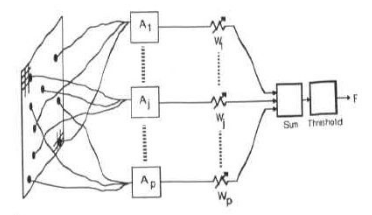
\includegraphics[width=0.5\textwidth]{perceptron.png}
\caption{Cấu trúc cơ bản của một perceptron \cite{minsky1969perceptron}}
\label{fig:perceptron}
\end{figure}

Như trong Hình \ref{fig:perceptron}, chúng ta có thể thấy perceptron nhận \textit{p} inputs, $A_1$, $A_2$, ..., $A_p$ (or $x_1$, $x_2$, ..., $x_p$, tùy thuộc vào nguồn.
Các yếu tố đầu vào sau đó được điều chỉnh theo trọng số $w_1$, $w_2$, ..., $w_p$, là những con số thực cho thấy tầm quan trọng của mỗi giá trị đầu vào.
Đầu ra \textit{F} sau đó sẽ được tính bằng cách sử dụng tổng của những đầu vào có trọng số đó. 
Ngoài ra, bởi vì đầu ra là một giá trị nhị phân, một ngưỡng được sử dụng để đạt được kết quả mong muốn. Để cụ thể hơn, một perceptron được viết như sau:

\begin{center}
$F = \begin{cases}
1 & if \sum_{i}^{p} A_i w_i \geq Threshold \\
0 & if \sum_{i}^{p} A_i w_i < Threshold
\end{cases}$
\end{center}

Do đó, đầu ra của một perceptron được điều khiển bởi hai điều: trọng số $w_1$, $w_2$, ..., $w_p$ và ngưỡng. 
Tuy nhiên, trong các mạng nơron hiện đại, phương trình đã thay đổi một chút bằng cách đưa Ngưỡng sang phía bên kia của bất phương trình.
Nghịch đảo phụ của Ngưỡng được gọi là Bias, và công thức sẽ được viết lại như sau:

\begin{center}
$F = \begin{cases}
1 & if \sum_{i}^{p} A_i w_i + Bias \geq 0 \\
0 & if \sum_{i}^{p} A_i w_i + Bias < 0
\end{cases}$
\end{center}

\subsubsection{Activation function}

Perceptron là tiền đề cho các artificial neuron hiện đại.
Thay vì chỉ trả về đầu ra nhị phân, artificial neuron bây giờ tạo ra các giá trị ở bất kỳ đâu trong phạm vi [0, 1].
Nguyên nhân chính là cải thiện qua trình học của một mạng.
Neural networks có thể học các tìm ra các trọng số và bias thích hợp cho đủ dữ liệu đầu vào. 
Quá trình học tập cần phải cải tiến, có nghĩa là trọng số và bias ngày càng gần với các giá trị càng tốt.
Chỉ có đầu ra nhị phân cho mỗi tế bào thần kinh khiến cho quá trình này khó thực hiện.
Để huấn luyện một neural network, chúng ta sử dụng một error function để xem cách xa hoặc đóng mạng là kết quả tối ưu hay không.
Do những đầu ra nhị phân của perception, một thay đổi nhỏ trong các tham số của mạng có thể dẫn đến sự khác biệt rõ rệt cho đầu ra, khiến cho việc điều chỉnh các tham số trở nên khó có thể đạt được kết quả tốt.
Do đó, sửa đổi phải được thực hiện cho mô hình perceptron gốc. 
Thay vì sử dụng 0 làm ngưỡng mà tại đó các tín hiệu được phép kích hoạt, chúng ta có thể sử dụng một hàm kích hoạt để ánh xạ đầu ra đến phạm vi mà chúng ta cần một cách thích hợp.

\begin{figure}[H]
\centering    
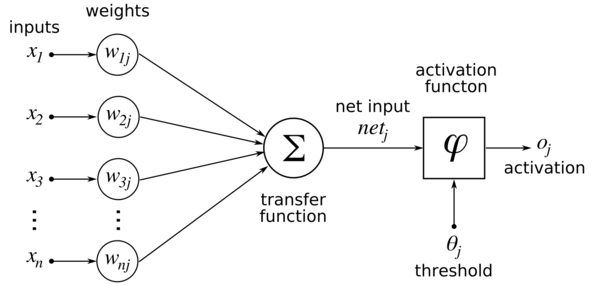
\includegraphics[width=0.7\textwidth]{artificial_neuron.png}
\caption{Cấu trúc của an artificial neuron \cite{wikian}}
\label{fig:artificial-neuron}
\end{figure}

Hàm kích hoạt lấy làm đầu vào tổng trọng số của các giá trị đầu vào được nạp vào perceptron và trả về một giá trị trong phạm vi [0,1]. 
Trong lịch sử, hàm Sigmoid được sử dụng cho mục đích này vì nó có thể cho ra output vào phạm vi mong muốn \cite{li2015cs231n}. 
Tuy nhiên những mạng bây giờ thì có dùng những hàm khác như là such as hyperbolic tan function (tanh) hoặc rectified linear unit (ReLU), để đạt hiệu năng tốt hơn \cite{li2015cs231n}.

\subsubsection{Feedforward và Backpropagation}

Hai hoạt động đặc biệt quan trọng trong neural networks: Feedforward và Backpropagation.

Feedforward được sử dụng trong cả giai đoạn đào tạo và thử nghiệm của mạng.
Nhiệm vụ chúng ta cần làm trong feedforward rất đơn giản: Truyền đầu ra của một lớp làm đầu vào của lớp tiếp theo.
Vì tất cả những gì chúng ta đang làm là một chiều đưa các giá trị qua mạng từ lớp đầu vào đến lớp đầu ra, hoạt động này được gọi là feedforward.

Backpropagation thường được sử dụng trong giai đoạn đào tạo để giúp các mạng nơron tìm hiểu các tham số của chúng, và nó được xem là một loại tối ưu hóa.
Khác với feedforward, công việc của thao tác này là truyền lỗi của các giá trị đầu ra trở lại mạng để cập nhật các tham số mạng.
Backpropagation hoạt động bằng cách đầu tiên thực hiện thao tác feedforward bình thường trên mạng với đầu vào đã cho.
Sau khi thu được đầu ra, chúng ta so sánh đầu ra với đầu ra mong muốn, sử dụng một loss function để tạo ra một error term cho mỗi nơron trong lớp đầu ra.
Các giá trị lỗi sau đó được truyền ngược từ lớp đầu ra cho đến khi tất cả các nơron nhận được error term tương ứng của chúng.
Các error term được sử dụng để tính gradient, cái mà chúng ta có thể cập nhật trọng số của mạng để giảm thiểu loss function khi quá trình lặp lại.
Để tìm các thông số phù hợp nhất, thuật toán gradient descent thường được áp dụng.

\section{Classification Metrics}

Trong phần này, chúng tôi xem xét cách sử dụng một số chỉ số phổ biến được sử dụng để đánh giá các dự đoán cho các vấn đề về phân loại.

\subsection{Logarithmic Loss}

Logarithmic loss, thường gọi tắt là log-loss, là chỉ số hiệu suất để đánh giá các dự đoán về xác suất đối với một lớp nhất định. Log-loss xem xét tính không chắc chắn của dự đoán dựa trên mức độ thay đổi của nó so với nhãn thực tế, điều này cho chúng ta cái nhìn sâu sắc hơn về hiệu suất của mô hình.
Trong phân loại nhị phân, với $y$ là chỉ báo nhị phân (0 hoặc 1) cho nhãn $c$ là phân loại chính xác và $p$ là mô hình dự đoán xác suất, công thức như sau:

\bigskip
\begin{center}
    $LogLoss = -(y\log(p) + (1 - y)\log(1 - p))$
\end{center}
\bigskip

Xác suất vô hướng giữa 0 và 1 có thể được xem như một thước đo sự tin cậy cho một dự đoán của một thuật toán.
Giá trị log-loss nhỏ hơn thì tốt hơn, và 0 thể hiện một log-loss hoàn hảo.

\subsection{Confusion Matrix}
\label{ssec:confusion_matrix}

\begin{figure}[H]
    \centering    
    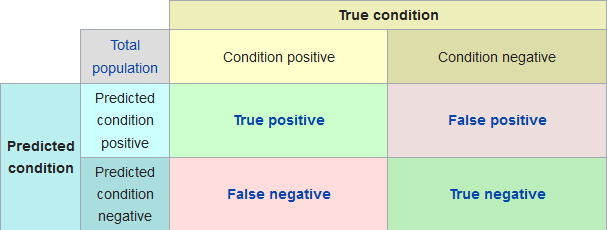
\includegraphics[width=0.7\textwidth]{confusion_matrix.png}
    \caption{Confusion matrix \cite{wiki_confusion_matrix}}
    \label{fig:confusion_matrix}
\end{figure}

Một cách rõ ràng để hiển thị kết quả dự đoán của một trình phân loại là sử dụng confusion matrix (còn được gọi là contingency table).
Đối với một vấn đề phân loại nhị phân, bảng có hai hàng và hai cột (được thể hiện trong hình \ref{fig:confusion_matrix}). 
Trên đầu là các nhãn lớp thực tế và xuống bên là các nhãn lớp được dự đoán.
Mỗi ô chứa số dự đoán được tạo bởi mô hình phân loại nằm trong ô đó.

\begin{figure}[H]
    \centering    
    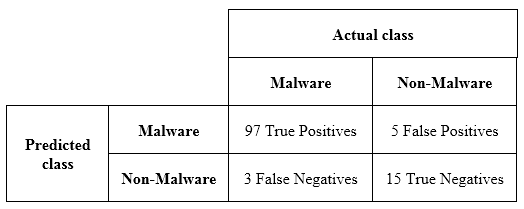
\includegraphics[width=0.7\textwidth]{confusion_matrix_example.png}
    \caption{Một ví dụ về confusion matrix}
    \label{fig:confusion_matrix_example}
\end{figure}

Hình \ref{fig:confusion_matrix_example} là một ví dụ về phân loại nhị phân trong phát hiện phần mềm độc hại.
Một số tệp đầu vào là phần mềm độc hại và thử nghiệm của chúng tôi chính xác cho biết chúng là có khả năng. Các kết quả đó gọi là true positives (TP). 
Ngược lại, khi chúng là malware, nhưng kết quả nói nó không phải. Chúng được gọi là false negatives (FN). 
Một số là tệp sạch và thử nghiệm cho biết chúng không phải là phần mềm độc hại – true negatives (TN). 
Cuối cùng, có thể có các tệp sạch sẽ có kết quả xét nghiệm dương tính - false positives (FP).

Có nhiều tỷ lệ xuất phát từ confusion matrix và các tỷ lệ phổ biến nhất được liệt kê dưới đây:

\begin{itemize}
    \item True Positive Rate (TPR), tương đương hit rate, recall: $TPR = TP/P = TP/(TP + FN)$
    \item True Negative Rate (TNR): $SPC = TN/N = TN/(TP + FN)$
    \item Precision hay Positive Predictive Value (PPV): $PPV = TP/(TP + FP)$
    \item Negative Predictive Value (NPV): $NPV = TN/(TN + FN)$
    \item Fall-out hay False Positive Rate (FPR): $FPR = FP/N = FP/(TP + FN) = 1 - TNR$
    \item False Discovery Rate (FDR): $FDR = FN/(FN + TP) = 1 - PPV$
    \item Miss Rate hay False Negative Rate (FNR): $FNR = FN/(FN + TP) = 1 - TPR$
\end{itemize}

\subsection{Độ chính xác tổng thể}

Độ chính xác tổng thể là tỉ lệ số dự đoán chính xác được thực hiện của tất cả các dự đoán được thực hiện.

\begin{center}
    ${Accuracy} =  \cfrac{True\ positive + True\ negative}{Condition\ positive + Condition\ negative}$
\end{center}
Độ chính xác tổng thể về cơ bản cho chúng ta biết tỷ lệ tất cả các dự đoán tham chiếu được ánh xạ chính xác.
Độ chính xác tổng thể thường được biểu thị bằng phần trăm, với độ chính xác 100\% là một phân loại hoàn hảo, trong đó tất cả các tham chiếu được phân loại chính xác.
Độ chính xác tổng thể là dễ hiểu và dễ tính toán nhất, nó cung cấp cho người dùng cái nhìn tổng quan về thông tin chính xác cần thiết.

Đây là chỉ số đánh giá phổ biến nhất cho các vấn đề phân loại, nó cũng là chỉ số dễ hiểu lầm nhiều nhất.
Nó chỉ phù hợp khi có số lượng quan sát ngang nhau trong mỗi lớp (hiếm khi xảy ra)và tất cả các dự đoán và sai số có tầm quan trọng như nhau(thường không phải là trường hợp phổ biến).

\subsection{Precision và Recall}

Precision có thể được coi như một thước đo về độ chính xác của bộ phân loại.
Precision cố gắng trả lời câu hỏi "Tỷ lệ nhận dạng tích cực thực sự chính xác là gì?".
Một precision thấy cũng có thể chỉ ra một số lượng lớn False Positives.

\begin{center}
    ${Precision} =  \cfrac{True\ positive}{True\ positive + False\ positive}$
\end{center}

Recall là số lượng True Positives chia cho tổng số lượng True Positives và False Negatives. Tính toán theo cách khác là số dự đoán tích cực chia cho số giá trị lớp dương trong dữ liệu thử nghiệm. Recall các nỗ lực để trả lời "Tỷ lệ tích cực thực tế đã được xác định chính xác?". Nó cũng tương đương Sensitivity hoặc True Positive Rate.

\begin{center}
    ${Recall} =  \cfrac{\sum True\ positive}{\sum Condition\ positive}$
\end{center}

\subsection{Diện tích dưới đường cong ROC}
\label{ssec:auroc}

Phần diện tích dưới đường cong ROC (Area Under the Receiver Operating Characteristic curve, AUROC hay AUC) là chỉ số hiệu suất cho các vấn đề phân loại nhị phân. AUROC có một số cách diễn giải tương đương:

\begin{itemize}
\item Kì vọng một uniformly drawn random positive xếp hạng trên một  a uniformly drawn random negative.
\item Tỉ lệ positives mong đợi xếp hạng trên một uniformly drawn random negative.
\item Tỉ lệ true positive rate mong đợi nếu việc xếp hạng được tách trước một a uniformly drawn random negative.
\item Tỉ lệ negatives mong đợi xếp hạng dưới niihr uniformly drawn random positive.
\item  Tỉ lệ false positive rate mong đợi nếu việc xếp hạng được tách sau một uniformly drawn random positive.
\end{itemize}

Diện tích $1,0$ đại diện cho một mô hình cho tất cả các dự đoán một cách hoàn hảo. Hệ thống điểm học thuật điển hình để phân loại độ chính xác là:

\begin{itemize}
\item 0.9 - 1.0 = Excellent
\item 0.8 - 0.9 = Good
\item 0.7 - 0.8 = Fair
\item 0.6 - 0.7 = Poor
\item 0.5 - 0.6 = Fail
\end{itemize}

\subsubsection{Cách tính AUROC}

Giả sử chúng ta có một mô hình phân lớp nhị phân là logistic regression. Đầu tiên, chúng ta tính hai thước đo từ confusion matrix (công thức của chúng được đề cập trong phần \ref{ssec:confusion_matrix}), sau đó sẽ được kết hợp thành một:

\begin{enumerate}
    \item \textbf{True positive rate (TPR).} Chỉ số này tương ứng với tỷ lệ các điểm dữ liệu tích cực được coi là dương, đối với tất cả các điểm dữ liệu tích cực. Nói cách khác, TPR càng cao hơn, càng ít các điểm dữ liệu tích cực chúng ta sẽ bỏ lỡ.
    \item \textbf{False positive rate (FPR).} Số liệu này tương ứng với tỷ lệ các điểm dữ liệu tiêu cực bị nhầm lẫn được coi là dương, liên quan đến tất cả các điểm dữ liệu tiêu cực. Nói cách khác, FPR cao hơn, các điểm dữ liệu tiêu cực sẽ bị phân loại sai.
\end{enumerate}

\begin{figure}[H]
    \centering    
    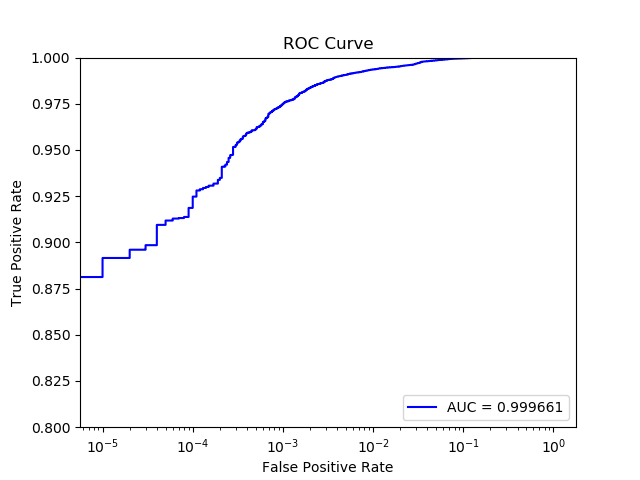
\includegraphics[width=0.8\textwidth]{roc_curve.png}
    \caption{Một ví dụ của đường cong Receiver Operating Characteristic}
    \label{fig:auroc}
\end{figure}

Sau đó, chúng ta kết hợp FPR và TPR vào một thước đo bởi việc tính toán hai thước đo này với những ngưỡng khác nhau (ví dụ, $0.00$, $10^-5$, $10^-4$, $10^-3$, ..., $1.00$, như trong hình \ref{fig:auroc})) và vẽ chúng trên một biểu đồ chung, với các giá trị FPR trên cạnh x và các giá trị TPR trên cạnh y. Đường cong có được gọi là Receiver Operating Characteristic curve, và giá trị thước đo của chúng ta chính là diện tích dưới đường cong ROC.

\section{LightGBM - A Gradient Boosting Framework}

LightGBM, có nghĩa là Light Gradient Boosting Machine, là một gradient boosting framework sử dụng tree-based learning algorithm \cite{ke2017lightgbm}. Framework đạt được sự phổ biến nhờ những ưu điểm sau:

\begin{itemize}
\item Tốc độ đào tạo nhanh hơn và hiệu quả cao hơn
\item Sử dụng ít bộ nhớ hơn
\item Độ chính xác tốt hơn
\item Hỗ trợ chạy song song và GPU
\item Hỗ trợ xử lý dữ liệu lớn
\end{itemize}

Framework sử dụng hai kỹ thuật sau đây để giải quyết vấn đề khi số lượng đặc trưng tăng cao và kích thước dữ liệu đáng kể: Gradient-based One-Side Sampling và Exclusive Feature Bundling.

\subsection{Gradient-based One-Side Sampling}

Dựa trên việc nhận thấy rằng, khi không có trọng số cho cá thể dữ liệu trong gradient-boosting decision tree, các cá thể dữ liệu với các gradient khác nhau đóng vai trò khác nhau trong việc thu thập thông tin (information gain).
Cụ thể, theo như định nghĩa của information gain, các cá thể với gradient lớn hơn (cụ thể là các cá thể đang được huấn luyện, under-trained instances) sẽ đóng góp nhiều hơn cho việc information gain.
Do đó, khi subsampling các cá thể dữ liệu, để đạt được độ chính xác dự tính của information gain, LightGBM có xu hướng giữ các cá thể với gradient lớn (ví dụ, lớn hơn một threshold định nghĩa trước, hoặc phần trăm phía trên), và chỉ loại bỏ ngẫu nhiên các cá thể có gradient nhỏ.
Họ đã chứng minh rằng hướng tiếp cận này dẫn đến một cách thu thập hiệu quả hơn việc uniformly random sampling, trong cùng một target sampling rate, đặc biệt là khi giá trị của information gain có một phạm vi rộng.

\subsection{Exclusive Feature Bundling}

Thông thường trong các ứng dụng thực tế, mặc dù có một lượng lớn các đặc trưng, không gian đặc trưng thường thưa thớt, cho phép LightGBM có khả năng sử dụng một cách tiếp cận gần như mất mát để giảm số lượng các đặc trưng.
Thực tế, trong một không gian đặc trưng thưa thớt, nhiều đặc trưng hầu như tách biệt, cụ thể, chúng hiếm khi cùng nhau bằng 0, ví dụ như những đặc trưng one-hot encoding, do đó, framework có thể đóng gói các đặc trưng tách biệt một cách an toàn.
LightGBM sử dụng một thuật toán hiệu quả gọi là Exclusive Feature Bundling, đây là một thuật toán tham lam với một tỷ lệ xấp xỉ không đổi.
Cụ thể, chúng chuyển optimal bundling problem thành a graph coloring problem bằng cách lấy các đối tượng như đỉnh và thêm cạnh cho mỗi hai đối tượng nếu chúng không cùng nhau độc quyền.